\documentclass{standalone}
\usepackage{pgfplots}
\pgfplotsset{compat=1.18}

\begin{document}

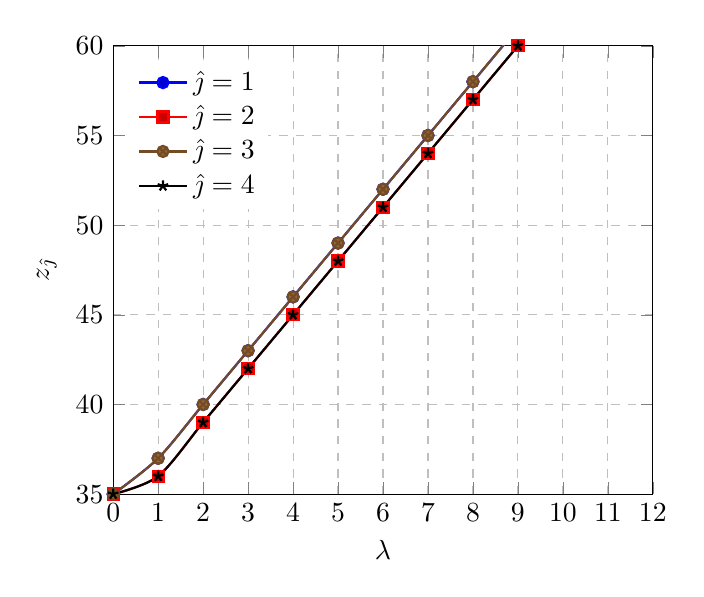
\begin{tikzpicture}
    \begin{axis}[
        xlabel=$\lambda$,
        ylabel=$z_{\hat{\jmath}}$,
        legend pos=north west,
        xmin=0, xmax=12,
        ymin=35, ymax=60,
        xtick={0,1,...,12},
        ytick={35,40,...,60},
        grid=major,
        grid style=dashed,
        legend entries={$\hat{\jmath}=1$, $\hat{\jmath}=2$, $\hat{\jmath}=3$, $\hat{\jmath}=4$},
        legend cell align=left,
        legend style={draw=none},
        smooth,
        every axis plot/.append style={thick},
        ]
        
        % Data for j=1
        \addplot coordinates {
            (0, 35) (1, 37) (2, 40) (3, 43) (4, 46) (5, 49) (6, 52) (7, 55) (8, 58) (9, 61) (10, 64) (11, 67)
        };
        
        % Data for j=2
        \addplot coordinates {
            (0, 35) (1, 36) (2, 39) (3, 42) (4, 45) (5, 48) (6, 51) (7, 54) (8, 57) (9, 60) (10, 63) (11, 66)
        };
        
        % Data for j=3
        \addplot coordinates {
            (0, 35) (1, 37) (2, 40) (3, 43) (4, 46) (5, 49) (6, 52) (7, 55) (8, 58) (9, 61) (10, 64) (11, 67)
        };
        
        % Data for j=4
        \addplot coordinates {
            (0, 35) (1, 36) (2, 39) (3, 42) (4, 45) (5, 48) (6, 51) (7, 54) (8, 57) (9, 60) (10, 63) (11, 66)
        };
        
    \end{axis}
\end{tikzpicture}

\end{document}